\chapter{DIZAJN I IMPLEMENTACIJA PIV SUSTAVA}
\label{chap:Poglavlje7}
U sklopu rada također je provedena implementacija i jednostavan pokazni primjer mjerenja koristeći PIV sustav. PIV sustav dizajniran je tako da omogući jednostavno korištenje, te minimalan napor za razumijevanje njegovog principa rada, što je i glavni cilj ovog rada u kojem se želi da budući korisnici što lakše poboljšaju znanje iz eksperimentalne i numeričke mehanike fluida. Također, PIV sustav je dizajniran modularno, s ciljem što manjih troškova, sa već dostupnom opremom unutar katedre fakulteta. Tipični komercijalni PIV sustavi danas su izuzetno skupi, sa cijenama od nekoliko desetaka tisuća eura, što dodatno otežava upoznavanje budućih generacija studenata sa PIV mjerenjima. Naravno, pri dizajniranju sustava moraju biti uzete mnoga pojednostavljenja, što limitira korištenje ovog sustava na samo određen broj  tipičnih strujanja (prvenstveno na strujanja u laminarnom području). Tip strujanja fluida ovisi o bezdimenzijskom broju poznatom kao Reynolds-ov broj:
\begin{equation}
	\Reyn = \dfrac{\rho v d}{\mu}
	\label{eqn:7.1}
\end{equation}
gdje $\rho$ označava gustoću fluida, $v$ karakterističnu brzinu strujanja, $d$ karakterističnu duljinu (za strujanje u cijevi, $d$ je promjer cijevi), te $\mu$ dinamičku viskoznost fluida. Pri niskim iznosima Reynolds-ovog broja strujanje teži laminarnom obliku (npr. $\Reyn \leq 2300$ za glatke cijevi), dok pri većim vrijednostima $\Reyn$ broja strujanje prelazi u tranzijentni, odnosno turbulentni oblik. Pri turbulentnom strujanju dolazi do slučajnih fluktuacija koje uzrokuju nepredvidive varijacije, što unosi nesigurnost u mjerenja brzine. Za takva mjerenja potreban je izuzetno robustan i skup, te često posebno dizajniran PIV sustav.\\
Kao što je već objašnjeno, glavne komponente PIV sustava su kamera, laser sa optikom, softver za analizu, te čestice markeri. Sa katedre fakulteta iskorištena je već dostupna brza kamera marke \textit{Chronos 1.4} (\textit{Slika \ref{sl:7.1}}) sa osnovnim karakteristikama rezolucije i fps-a prikazanim u \textit{Tablici \ref{tab:7.1}}. 
\begin{figure}[h]  
	\centering
	%\usepackage{graphicx}
	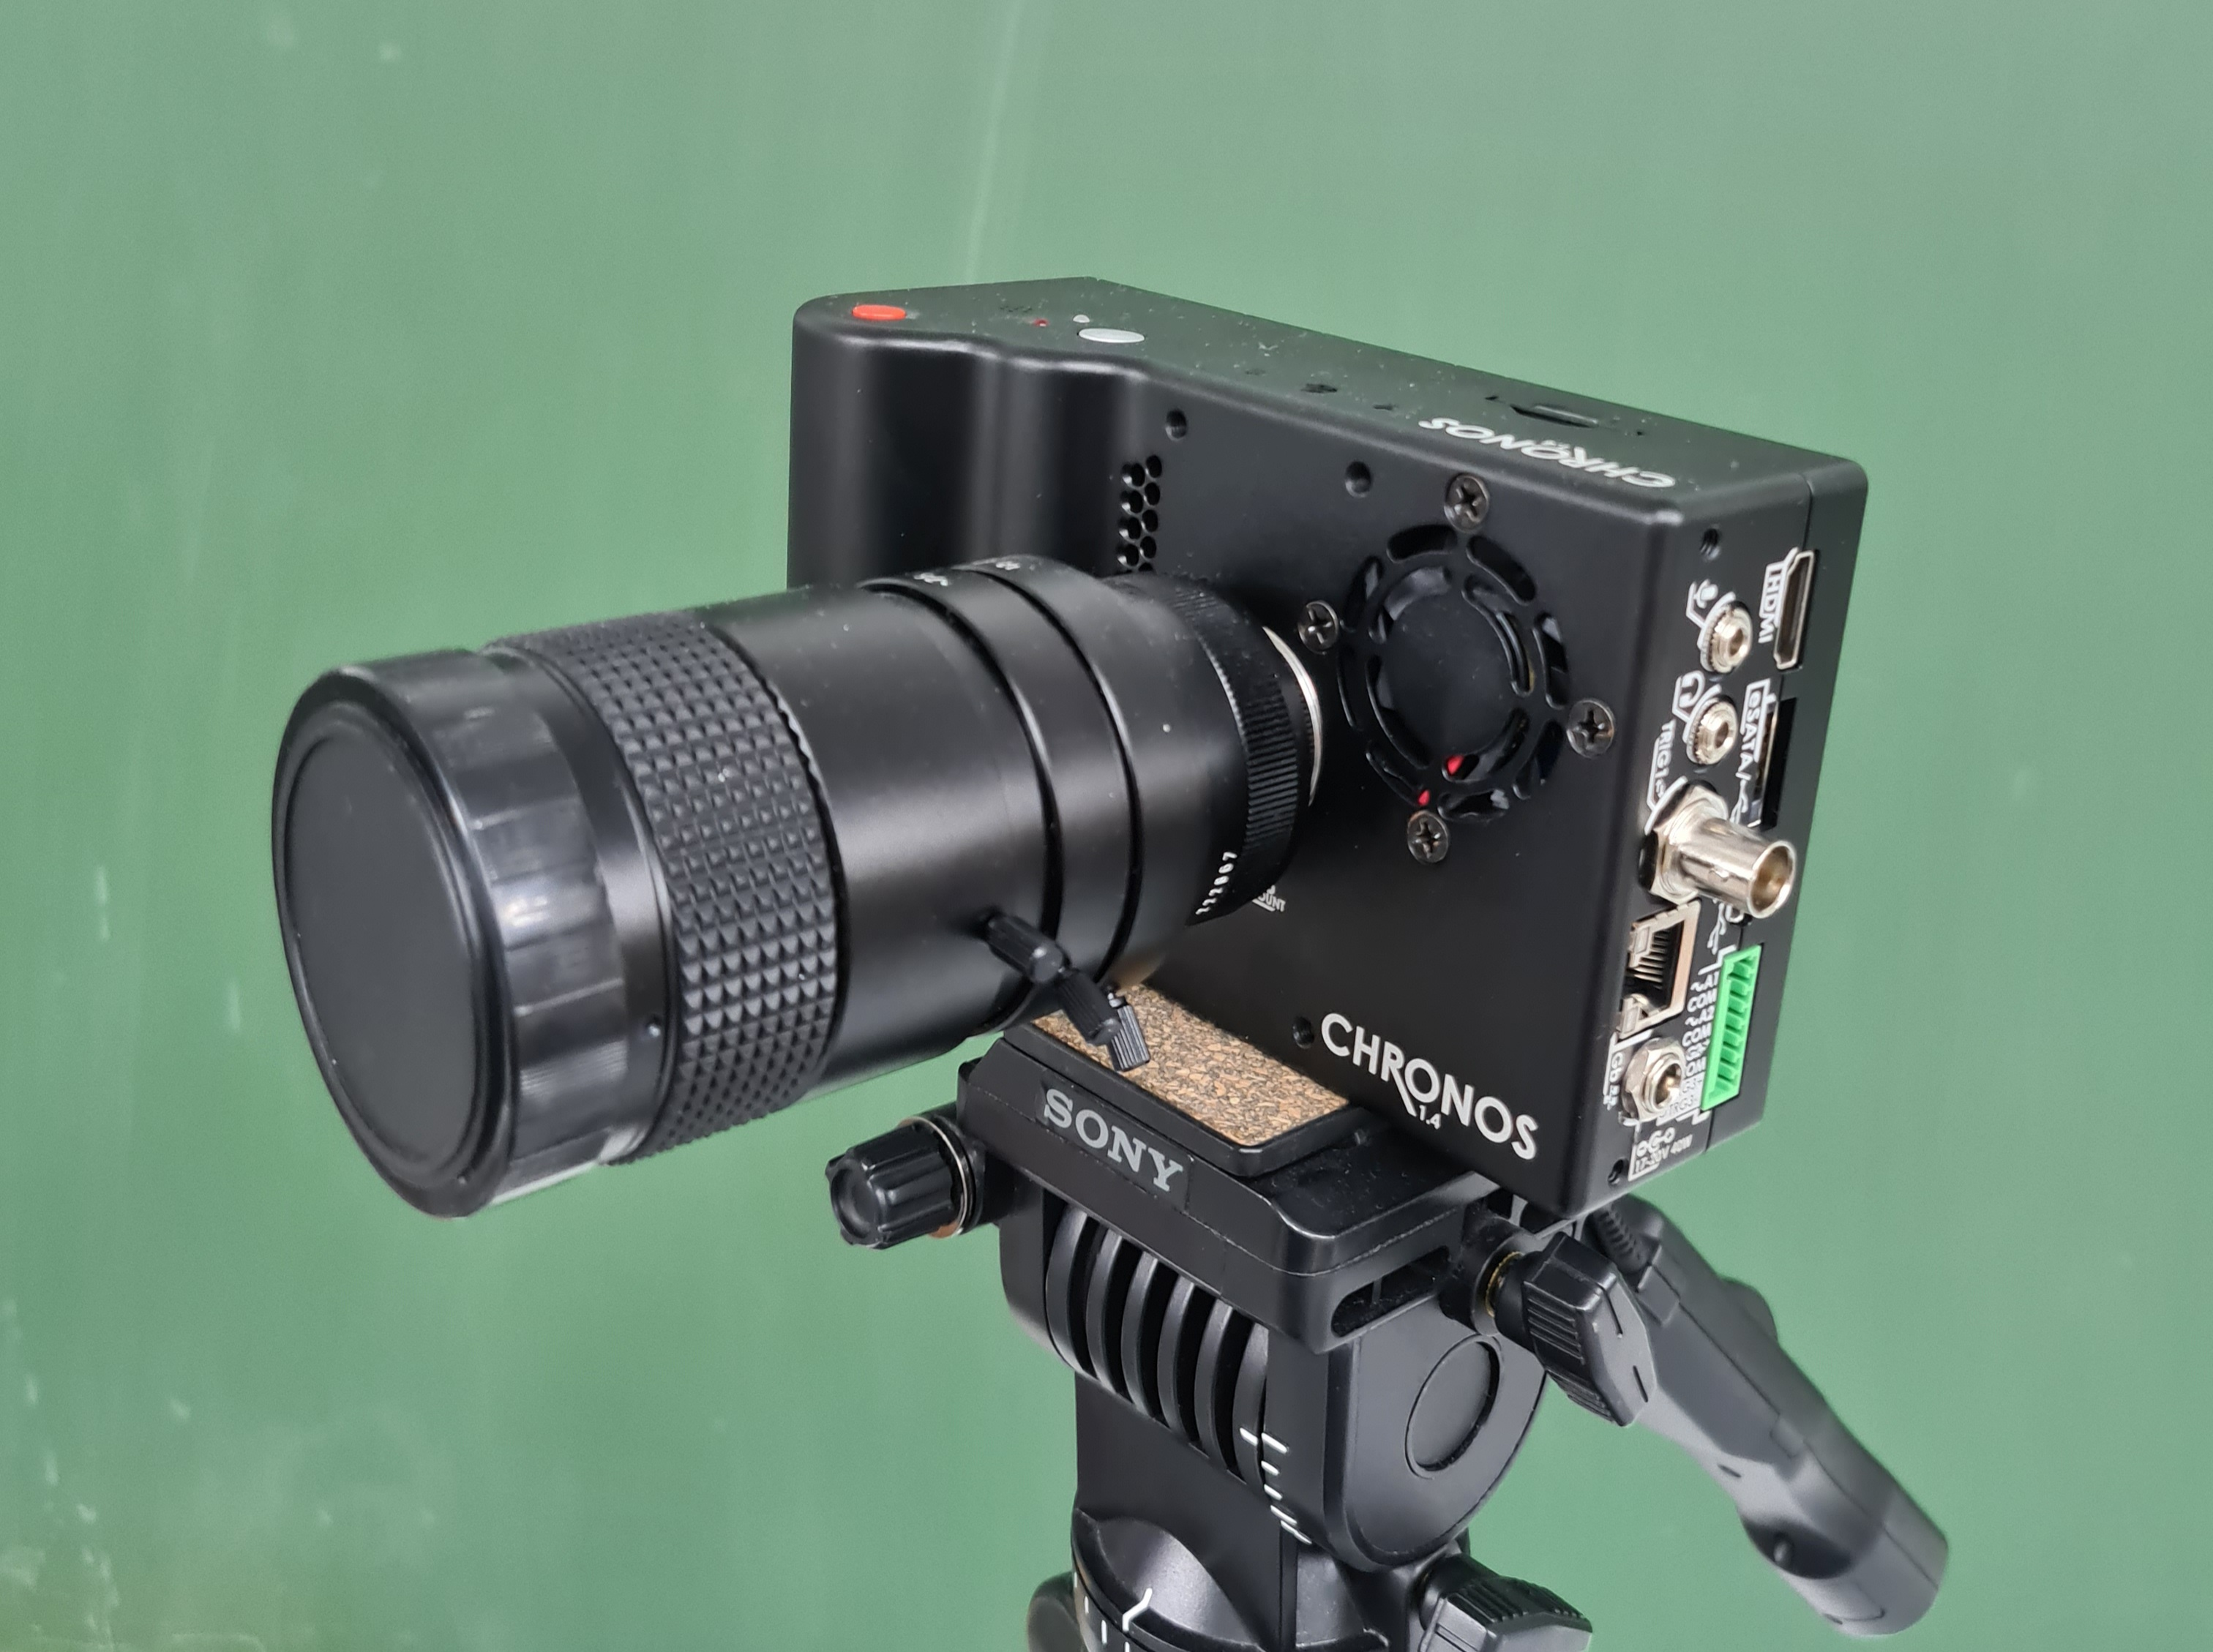
\includegraphics[width=7.4cm]{./7_LowCostPIV/slika7_1.jpg} 
	\caption{Chronos 1.4 brza kamera}
	\label{sl:7.1}
\end{figure}
\par
Kvalitetna kamera u suštini je najbitnija komponenta PIV sustava, te korištena kamera je izuzetno robusna i moguće ju je koristiti kod raznih tipova strujanja uz dodatnu optimizaciju ostalih parametara sustava. Chronos 1.4 je lako prijenosna brza kamera, te ima mogućnost snimanja videozapisa rezolucije $1280\times1024$ pri $1057$ fps-a, a može snimati do $38500$ fps-a pri nižoj razlučivosti. Video se sprema u komprimirani h.264 format ili nekomprimirani RAW format na prijenosni medij (memorijska microSD kartica).
\begin{table}[h]
	\centering
	\caption{Rezolucija i maksimalni broj fps-a za Chronos 1.4 kameru}
	\begin{tabular}{ccc}
		\rowcolor[HTML]{C0C0C0} 
		\textbf{Rezolucija} & \textbf{\begin{tabular}[c]{@{}c@{}}Maks. \\ fps\end{tabular}} & \textbf{\begin{tabular}[c]{@{}c@{}}Vrijeme snimanja \\ (sek.) - 8GB\end{tabular}} \\ \hline
		$1280\times1024$    & 1 057                                                         & 4.13                                                                              \\
		$1280\times720$     & 1 502                                                         & 4.13                                                                              \\
		$1280\times512$     & 2 111                                                         & 4.14                                                                              \\
		$1280\times360$     & 2 999                                                         & 4.14                                                                              \\ \hline
		$1280\times240$     & 4 489                                                         & 4.15                                                                              \\
		$1280\times120$     & 8 923                                                         & 4.17                                                                              \\
		$1280\times96$      & 11 119                                                        & 4.19                                                                              \\
		$1024\times768$     & 1 771                                                         & 4.11                                                                              \\ \hline
		$1024\times576$     & 2 359                                                         & 4.11                                                                              \\
		$800\times600$      & 2 873                                                         & 4.15                                                                              \\
		$800\times480$      & 3 587                                                         & 4.15                                                                              \\
		$640\times480$      & 4 436                                                         & 4.20                                                                              \\ \hline
		$640\times360$      & 5 903                                                         & 4.21                                                                              \\
		$640\times240$      & 8 816                                                         & 4.23                                                                              \\
		$640\times120$      & 17 424                                                        & 4.28                                                                              \\
		$640\times96$       & 21 649                                                        & 4.30                                                                              \\ \hline
		$336\times252$      & 15 200                                                        & 4.43                                                                              \\
		$336\times190$      & 20 020                                                        & 4.47                                                                              \\
		$336\times120$      & 31 192                                                        & 4.53                                                                              \\
		$336\times96$       & 38 565                                                        & 4.60                                                                             
	\end{tabular}
\label{tab:7.1}
\end{table}
\par
Za potrebe laserskog osvjetljenja nabavljen je niskobudžetni laserski modul \textit{CW532-050L} (\textit{Slika \ref{sl:7.2}}). \textit{CW532-050L} je DPSS (diodno upumpavani laser sa čvrstom jezgrom) laserski modul kompaktne veličine koji na sebi ima ugrađenu optiku za generiranje ravnine (linije) pod kutom od 60°. Emitira na valnoj duljini od 532 nm što odgovara zelenoj svjetlosti, te ima optičku izlaznu snagu od 50 mW i automatsku kontrolu snage. Promjer zrake na otvoru (prije linijske optike) iznosi 1.5 mm, te zraka ima divergenciju u iznosu od 1.2 mrad. Optika za generiranje linije je 2'' cilindrična staklena leća. Opisani laser je odabran zbog jednostavnog upravljanja i korištenja koje jedino zahtjeva dodatno napajanje i ponor topline, te je preporučeno korištenje zaštite za vid pri rukovanju sa laserom. Laser također emitira kontinuiranu zraku, pa nije potreban uređaj za sinkronizaciju "puls-eva" lasera i kamere.
\begin{figure}[h]  
	\centering
	%\usepackage{graphicx}
	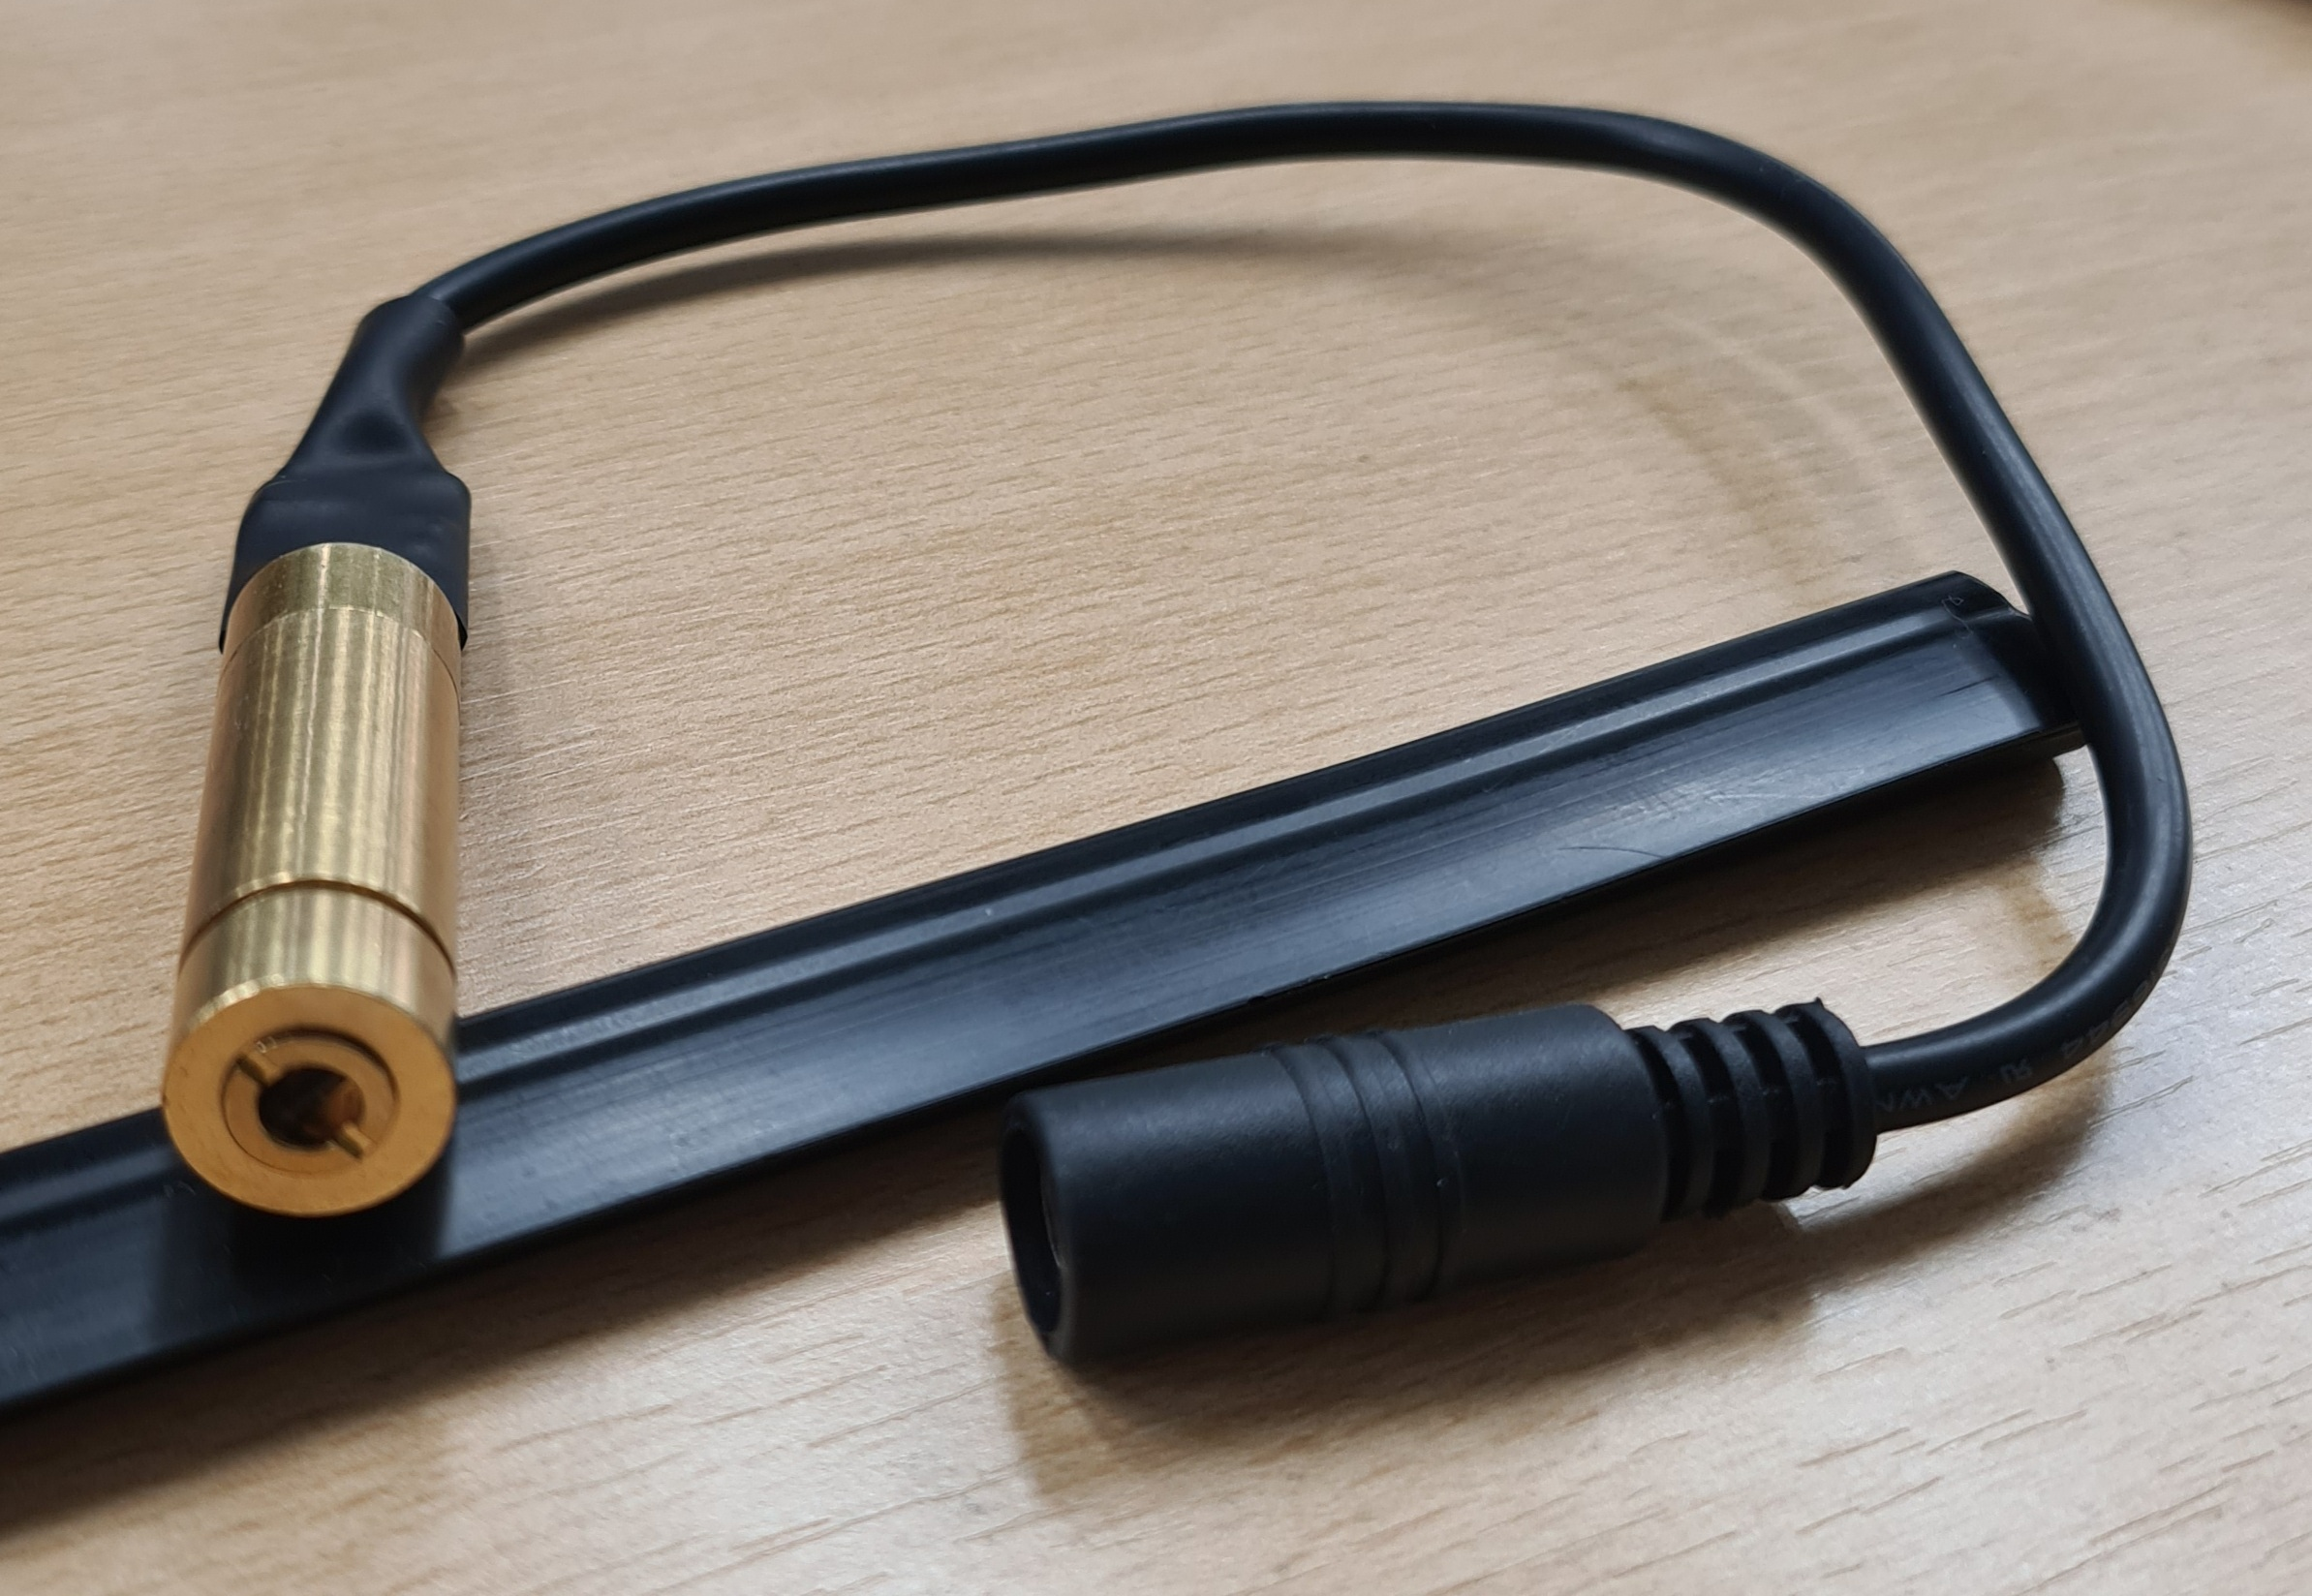
\includegraphics[width=9cm]{./7_LowCostPIV/slika7_2.jpg} 
	\caption{CW532-050L DPSS zeleni laser sa ugrađenom linijskom optikom}
	\label{sl:7.2}
\end{figure}
\par
Kako je dizajniran 2D PIV sustav, kao softver za analizu korišten je PIVlab koji u sebi ima uključene najnovije (\textit{eng. state od the art}) tehnike obrade slike i podataka. Za korištenje PIVlab softvera potrebna je MATLAB licenca koju mnoga sveučilišta obično posjeduju, ali moguće je korištenje i putem studentske licence u vrijednosti cca. 100 \$. Kao što je već ranije opisano PIV mjerenja se obično izvode u vodi ili zraku, pri čemu je u promatrane fluide potrebno dodati čestice markere od kojih će se odbijati laserska svjetlost, te tako označiti strujanje. Pri testnom mjerenju u ovom radu nisu korištene dodatne čestice zbog korištenja vode iz slavine u kojoj već postoje sitne čestice kamenca koje su bile sasvim dovoljne za vizualizaciju strujanja. Naravno, za bilo kakva ozbiljnija mjerenja potrebno je ispravno odabrati čestice markere, te kao preporuku niskobudžetnih čestica moguće je koristiti npr. sitne otpadne čestice pri CNC obradi (za mjerenja u vodi), ili čestice finog škroba (za mjerenja u zraku).
\par
Kao testni pokazni primjer funkcioniranja PIV eksperimenta izabrano je mjerenje brzine istrujavanja iz cijevi promjera 4 mm u spremnik kvadratnog oblika dimenzija $200\times200\times500$ mm (\textit{Slika \ref{sl:7.3}}). U spremnik je dodana voda iz slavine, te je uronjena cijev iz koje istrujava voda, koja se pumpa iz drugog spremnika. Brzina istrujavanja iz cijevi iznosi cca. 3 m/s (nisu uračunati gubici), dok volumni protok pumpe iznosi cca. 2.4 l/min. Kraj cijevi je vertikalno uronjen u vodu, te je laserska ravnina postavljena tako da cijev uzdužno siječe na pola kao što je vidljivo na slici.
\begin{figure}[h]  
	\centering
	%\usepackage{graphicx}
	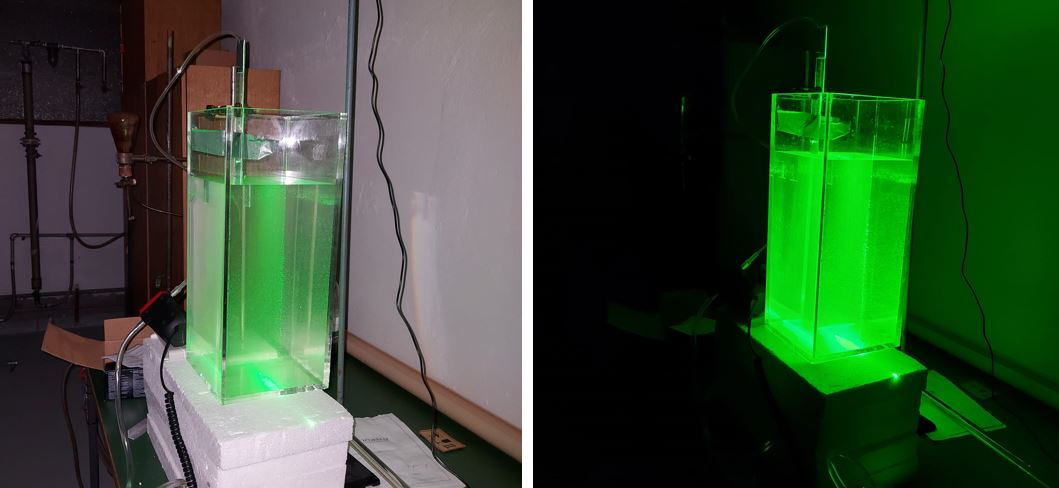
\includegraphics[width=15cm]{./7_LowCostPIV/slika7_3.jpg} 
	\caption{Izgled postavljenog testnog mjerenja}
	\label{sl:7.3}
\end{figure}
\par
Kamera je postavljena normalno na lasersku ravninu, te je namještena najviša moguća rezolucija ($1280\times1024$). Kao brzina stvaranja slike odabrano je 500 fps-a, pokušano je i snimanje sa većim brojem fps-a, ali lasersko osvjetljenje iznad 500 fps-a nije dovoljno snažno da ispravno osvijetli čestice zbog prekratke duljine ekspozicije, te dobivene snimke zbog prevelike količine šuma nisu bile upotrebljive za kros-korelacijsku analizu. Na mjestu gdje laserska ravnina obasjava spremnik postavljena je i mjerna skala koja služi u kasnijoj kalibraciji stvarne duljine domene i duljine domene u ravnini slike (\textit{Slika \ref{sl:7.4}}).
 \begin{figure}[h]  
 	\centering
 	%\usepackage{graphicx}
 	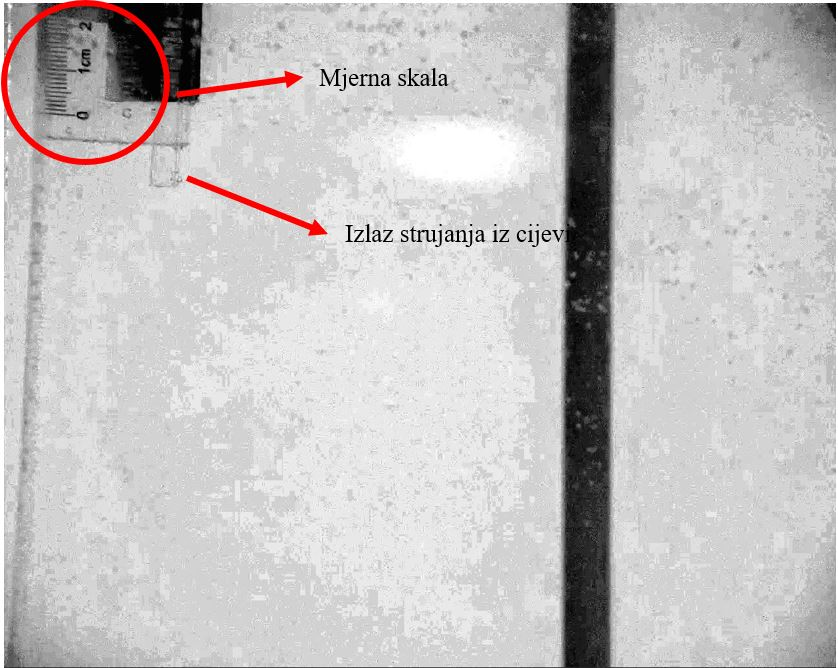
\includegraphics[width=8cm]{./7_LowCostPIV/slika7_4.jpg} 
 	\caption{Kalibracijska snimka kojom se povezuje veličina stvarne domene sa veličinom domene u ravnini slike}
 	\label{sl:7.4}
 \end{figure}
\par
Nakon snimanja akvizicije snimki slijedi prijenos snimki na vanjsku memoriju (microSD) te konačno pohranjivanje na memoriju računala u kojem će se vršiti kros-korelacijska analiza. Prije pokretanja PIVlab programa, uz pomoć open-source VirtualDUB softvera \cite{virtualdub} izvučeno je 50 kadrova (snimke) koje se obliku .mp4 formata u ovom slučaju učitavaju u PIVlab softver.
\begin{description}[style=unboxed,leftmargin=0cm]
	\item[Pretprocesiranje snimki] Kao što je već ranije opisano, PIVlab omogućuje nekoliko tehnika obrade slike kojima se osjetno poboljšati kvaliteta kros-korelacijske analize. Prema zadanim postavkama omogućena je CLAHE tehnika koja lokalno poboljša kontrast u slikama. Također izračunata je prosječna vrijednost pozadine svih 50 kadrova (\textit{Slika \ref{sl:7.6}b}), te je oduzeta od svake snimke posebno što značajno poveća kontrast snimki. Ostale postavljene tehnike prikazane su na \textit{Slici \ref{sl:7.5}}, te je na \textit{Slici \ref{sl:7.6}a} prikazan izgled neobrađene snimke, dok je na \textit{Slici \ref{sl:7.6}c} vidljiv konačan rezultat primjene pretprocesorskih tehnika. Također na \textit{Slici \ref{sl:7.6}c} vidljivo je crveno područje koje je isključeno iz kros-korelacijske analize jer u tom području nema strujanja.
	 \begin{figure}[h]  
		\centering
		%\usepackage{graphicx}
		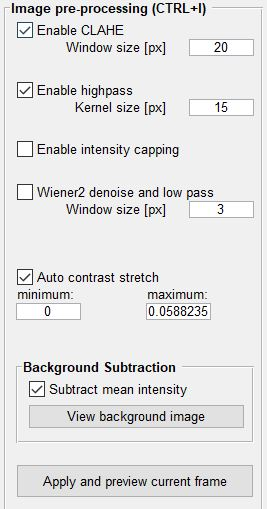
\includegraphics[width=5.5cm]{./7_LowCostPIV/slika7_5.jpg} 
		\caption{Postavljene postavke pretprocesiranja slike u PIVlab softveru}
		\label{sl:7.5}
	\end{figure}
	\begin{figure}[h]  
		\centering
		%\usepackage{graphicx}
		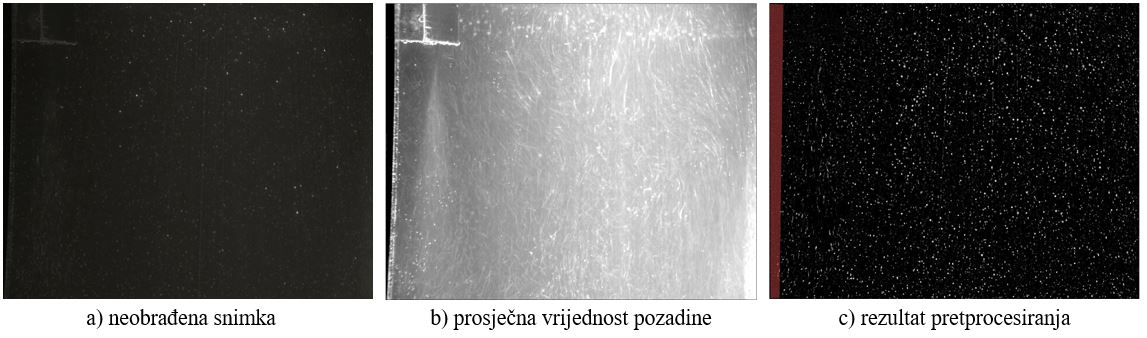
\includegraphics[width=16.5cm]{./7_LowCostPIV/slika7_6.jpg} 
		\caption{Izgled dobivenih snimki: na slici a) prikazana je neobrađena PIV snimka, slika b) prikazuje prosječnu vrijednost pozadine 50 kadrova koji se analiziraju, te se ti kadrovi oduzmu od slike a), dok slika c) prikazuje konačan rezultat obrade snimki}
		\label{sl:7.6}
	\end{figure}
	\item[Opcije PIV analize] PIVlab ima tri različita korelacijska algoritma: DKK (direktnu kros-korelaciju u jednom prolazu), korelaciju skupine snimki (\textit{eng. Ensemble correlation}), te FFT sa tehnikom deformacije prozora. Prema zadanim postavkama omogućen je FFT sa tehnikom deformacije prozora, prvenstveno zbog toga što u većini situacija daje najbolje rezultate. Ovaj algoritam korišten je i u analizi učitanih snimki, te se snimke njime analiziraju u nekoliko prolaza. 
	\begin{figure}[h]  
		\centering
		%\usepackage{graphicx}
		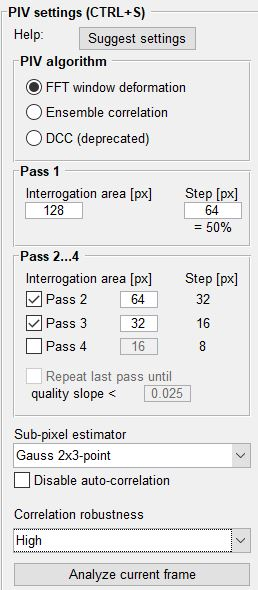
\includegraphics[width=5cm]{./7_LowCostPIV/slika7_7.jpg} 
		\caption{Odabrane postavke za kros-korelacijsku analizu}
		\label{sl:7.7}
	\end{figure}
	\par
	Preporuka je da u prvom prolazu se koristi relativno velik prozor ispitivanja kako bi se pouzdano izračunao pomak podataka sa snimke, jer kao što je već ranije opisano veći prozor ispitivanja daje i veći omjer signala i šuma, te samim time i bolju kros-korelacijsku analizu. Cijena korištenja većih prozora ispitivanja je manja rezolucija vektora brzina, pa je zbog toga korištenje FFT tehnike deformacije prozora mnogo robusnije od ostalih tehnika. Naime u sljedećim prolazima, uzima se manja veličina prozora ispitivanja, te se koriste informacije od prethodnog prolaza kako bi se pomaknulo ispitivanje ("deformiralo" područje ispitivanja) u trenutnom prolazu. Na taj način poveća se vektorska rezolucija (viši DVR), te omjer signala i šuma. Generalna preporuka je korištenje barem 3 prolaza, te nije bitno da oni budu djeljivi sa dva jer MATLAB za korelaciju koristi FFTW koji može "rukovati" sa proizvoljnim veličina prozora ispitivanja. Bitno je samo da se prozori ispitivanja postepeno smanjuju sa brojem prolaza. Također potrebno je napomenuti kako postavljanje iznimno malenog prozora ispitivanja u posljednjem prolazu (npr. $4\times4$ pixela), dovodi do osjetnog smanjenja omjera signal-šum, što dovodi do nesigurnosti u mjerenju, te je zbog toga potrebno oprezno postaviti veličinu posljednjeg prozora ispitivanja. Na \textit{Slici \ref{sl:7.7}} prikazane su korištene postavke pri testnom mjerenju u ovom radu.
	\item[Kalibracija] Nakon analize snimki PIVlab kao jedinicu pomaka koristi "pixel po kadru" (\textit{eng. pixel per frame}), te je potrebna kalibracija kojom se laički softveru kaže koliko se pixela nalazi u jedinici mjere (npr. u metrima), te se zada vremenski korak između kadrova snimki. Na \textit{Slici \ref{sl:7.8}} prikazane su odabrane kalibracijske postavke mjerenja. Odabran je pozitivan smjer x-osi udesno, te pozitivan smjer y-osi prema gore. Na \textit{Slici \ref{sl:7.4}} dodijeljen je razmak od 20 mm pomoću PIVlab grafičkog sučelja i mjerne skale na kalibracijskoj snimci, te je odabran vremenski korak od 2 milisekunde, što odgovara stvaranju snimki pri 500 fps-a. Mjerna skala postavljena je u ravnini laserskog osvjetljenja, te se jednostavno uz pomoć nje povežu stvarne duljina u ravnini lasera i duljina u ravnini slike.
	\begin{figure}[h]  
		\centering
		%\usepackage{graphicx}
		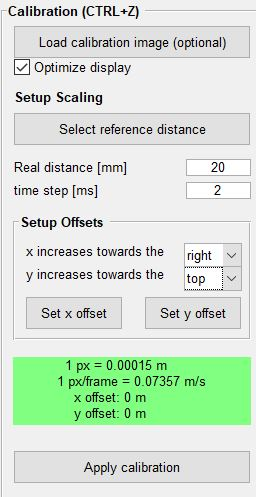
\includegraphics[width=5cm]{./7_LowCostPIV/slika7_8.jpg} 
		\caption{Odabrane postavke za kalibraciju PIV snimki}
		\label{sl:7.8}
	\end{figure}
	\item[Validacija dobivenih podataka] Kako su ovom radu napravljena pokusna testna mjerenja, gdje nisu sasvim dovoljno dobro optimizirani vanjski parametri mjerenja, ovo poglavlje služi kao pokazni primjer pripreme i realizacije PIV eksperimenta. Radi navedenih razloga prilikom kros-korelacijske analize dobiveno je dosta nepravilnih vektora koje je potrebno validirati, te kasnije aproksimirati i zamijeniti što realnim podacima. PIVlab softver ima dvije opcije filtriranja podataka: validacija temeljena na brzini strujanja (\textit{eng. Velocity based validation}), te validaciju temeljenu na podacima sa slike (\textit{eng. Image based validation}). Obično je prilikom provjere dovoljna samo validacija temeljena na brzini gdje se u suštinu odredu gornja i donja granica vrijednosti x i y komponenti brzine. Prilikom odabiranja postavki validacije u ovom radu zadano je samo da lokalne razlike između susjednih vektora brzina budu što manje, tj. zadana je dinamička provjera razlike vektora, tako da je odabrana strogoća filtra brzine iz jednadžbe \ref{eqn:2.10} i \ref{eqn:2.11} u iznosu od 8.
\end{description}
Na sljedećim slikama prikazani su rezultati mjerenja pri 500 fps-a. Na \textit{Slici \ref{sl:7.9}} je vidljivo je dobiveno polje brzina u PIVlab softveru. Kako bi brzina istrujavanja iz cijevi u gornjem lijevom kutu trebala biti cca. 3 m/s jasno je kako korelacijski algoritam nije uspio dobiti dobre brzine. Razlog tome je prvenstveno u previše nasumičnom i turbulentnom 3D istrujavanju iz cijevi. Naime prilikom istrujavanja previše čestica napušta osvijetljenu ravninu te dolazi do prekomjernog izvan-ravninskog gibanja, u kojem se između kadrova gube parovi čestica i korelacijski algoritam ostaje bez uzoraka koje bi trebao povezati. Nadalje kako prilikom mjerenja nisu korištene čestice markeri, nego se na snimkama vide osvijetljene čestice kamenca koje nemaju uniformnu gustoću distribucije, te imaju prevelike razlike u veličini jasno je da dobiveni podaci teško mogu odražavati pravu sliku strujanja, te bilo kakva relevantna mjerenja nisu moguća bez dodavanja čestica markera.
\begin{figure}[h]  
	\centering
	%\usepackage{graphicx}
	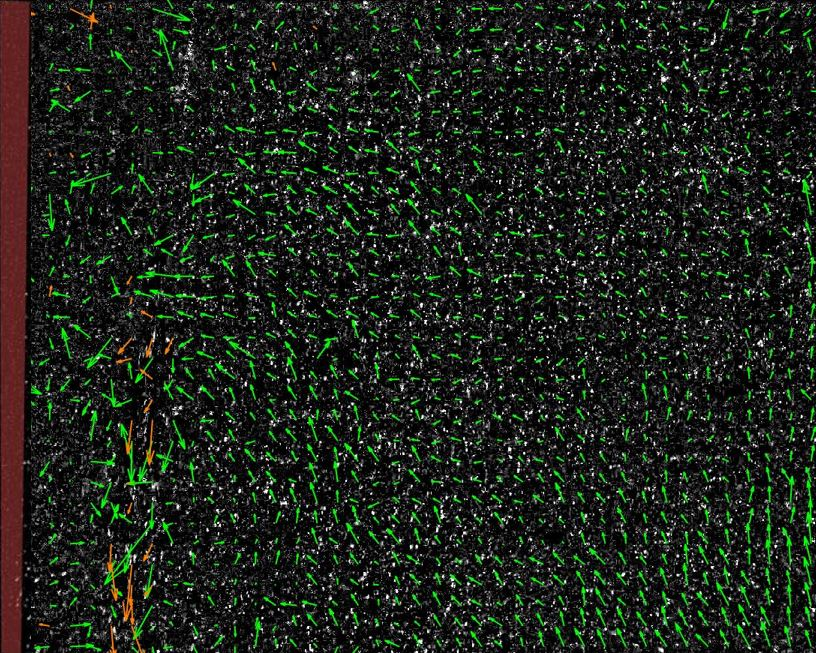
\includegraphics[width=10cm]{./7_LowCostPIV/slika7_9.jpg} 
	\caption{Dobiveno polje brzina u PIVlab softveru (zelenom bojom su označeni izmjereni vektori, a narančastom interpolirani vektori)}
	\label{sl:7.9}
\end{figure}
\par
Dodatni razlog loših rezultata u području istrujavanja je i neujednačena, te jako neuniformna distribucija osvijetljenje u ravninskom smjeru, te u smjeru normalnom na lasersku ravninu. Naime korišteni nisko-budžetni laser nakon samo kratkog rada, osjetno gubi svojstva, te dobivanje što kvalitetnijih mjerenja čini dodatno težim. No ipak rezultati izvan zone istrujavanja čine se dosta boljima i realnijima. Kako je usporenje slojeva vode unutar spremnika dosta intenzivno, dobivene niske brzine u PIV mjerenjima koliko-toliko dosta realnije opisuju polje brzina unutar spremnika. Dobivene komponente brzina u x i y smjeru, moguće je vidjeti na \textit{Slici \ref{sl:7.10}} na $u$-$v$ dijagramu. Iz dijagrama je jasno kako većina $u$ komponenti vektora ima vrijednost između -0.15 m/s i 0.1 m/s, dok $v$ komponenta ide od -0.1 m/s do 0.15 m/s. Dodatni razlog tako niskih brzina je moguća pojava vrtloga na mjestu istrujavanja. Vrtlog se širi u smjeru okomito na snimku te je moguće kako on dodatno prigušuje brzine unutar domene.
\begin{figure}[h]  
	\centering
	%\usepackage{graphicx}
	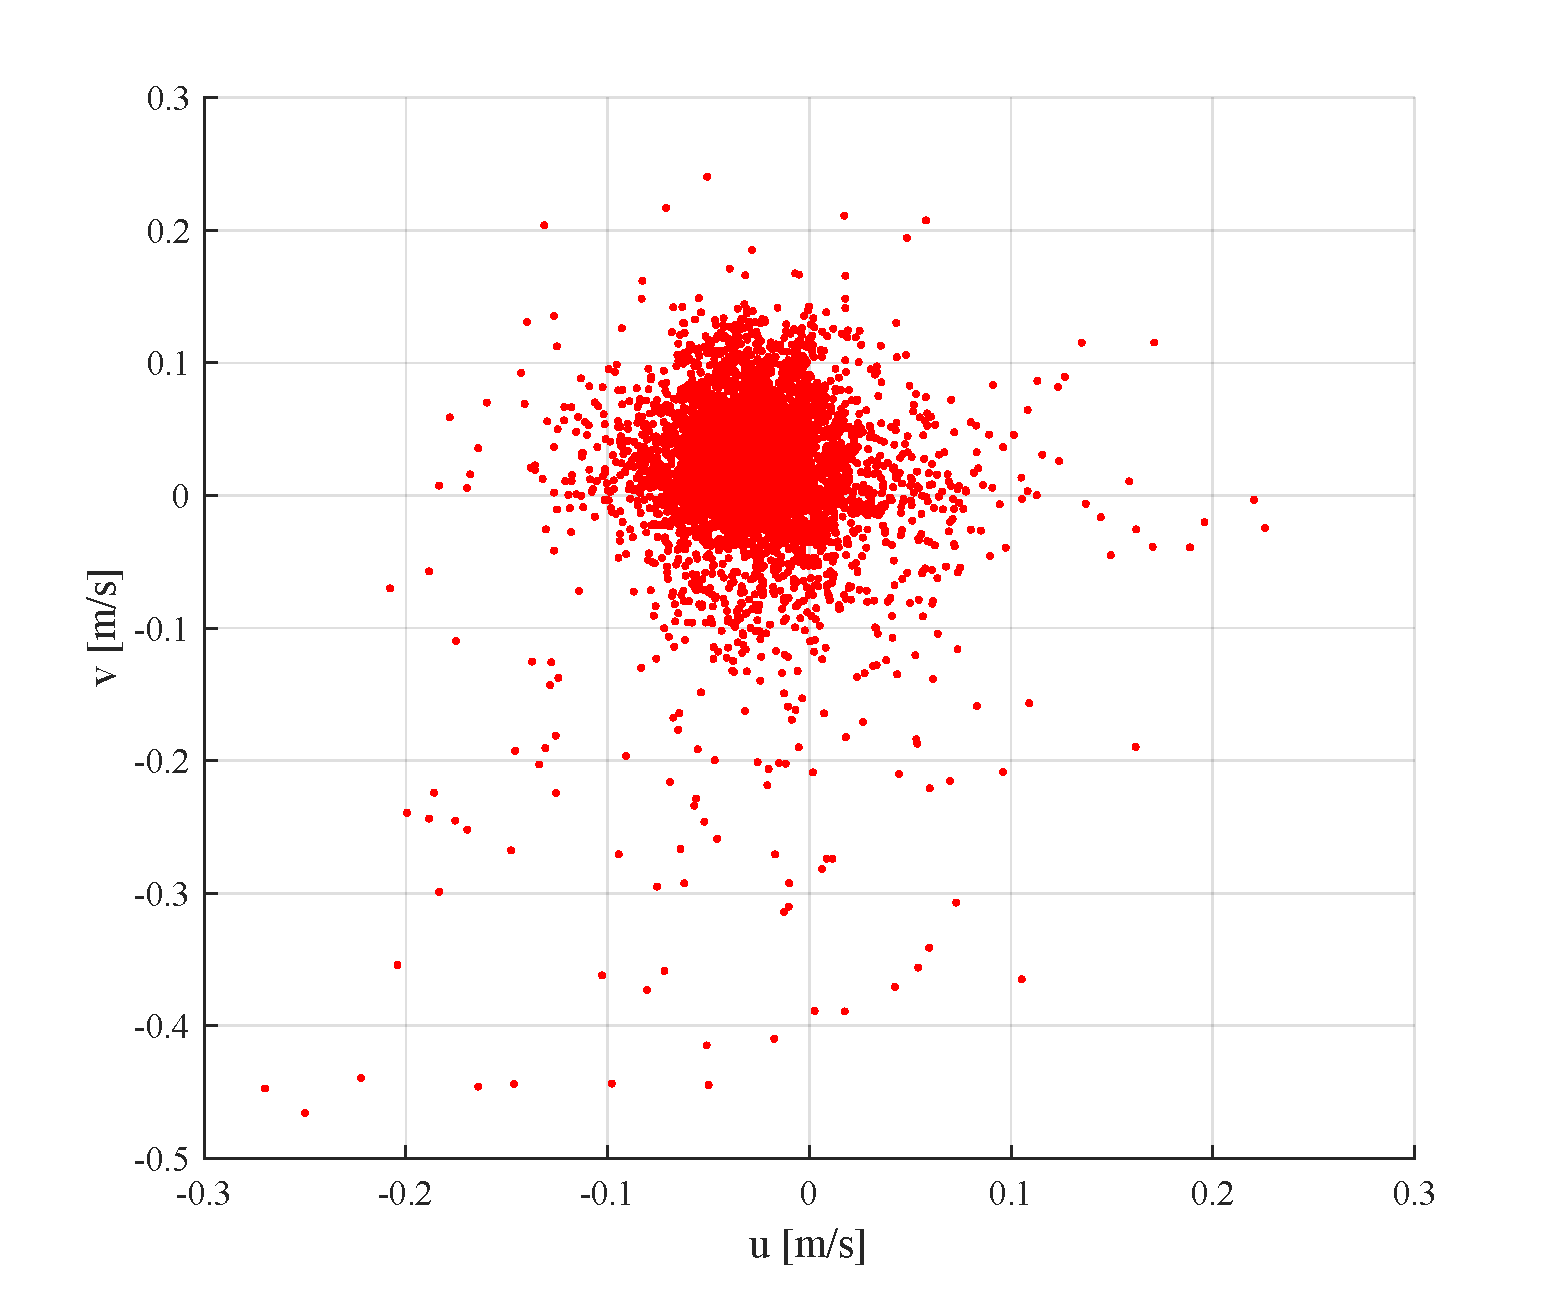
\includegraphics[width=10cm]{./7_LowCostPIV/slika7_10.pdf} 
	\caption{Dobiveni rezultati - $u$-$v$ "scatter" dijagram}
	\label{sl:7.10}
\end{figure}
\par
Na \textit{Slici \ref{sl:7.11}} prikazan je histogram ukupne brzine, te je vidljivo kako najučestaliju frekvenciju pojavljivanja ima brzina malo veća od 0.05 m/s. Ove dobivene podatke jasnije bi trebalo provjeriti sa puno robustnijim PIV sustavom, koji u ovom diplomskom radu nije bilo moguće izvesti, a u suštini to nije bio ni cilj rada. Dodatna provjera rezultata mogla bi  se provesti uz pomoć CFD analize, koja bi uz kvalitetno postavljene parametre simulacije zasigurno mogla omogućiti bolji "osjećaj" za veličine brzina u promatranom strujanju.
\begin{figure}[h]  
	\centering
	%\usepackage{graphicx}
	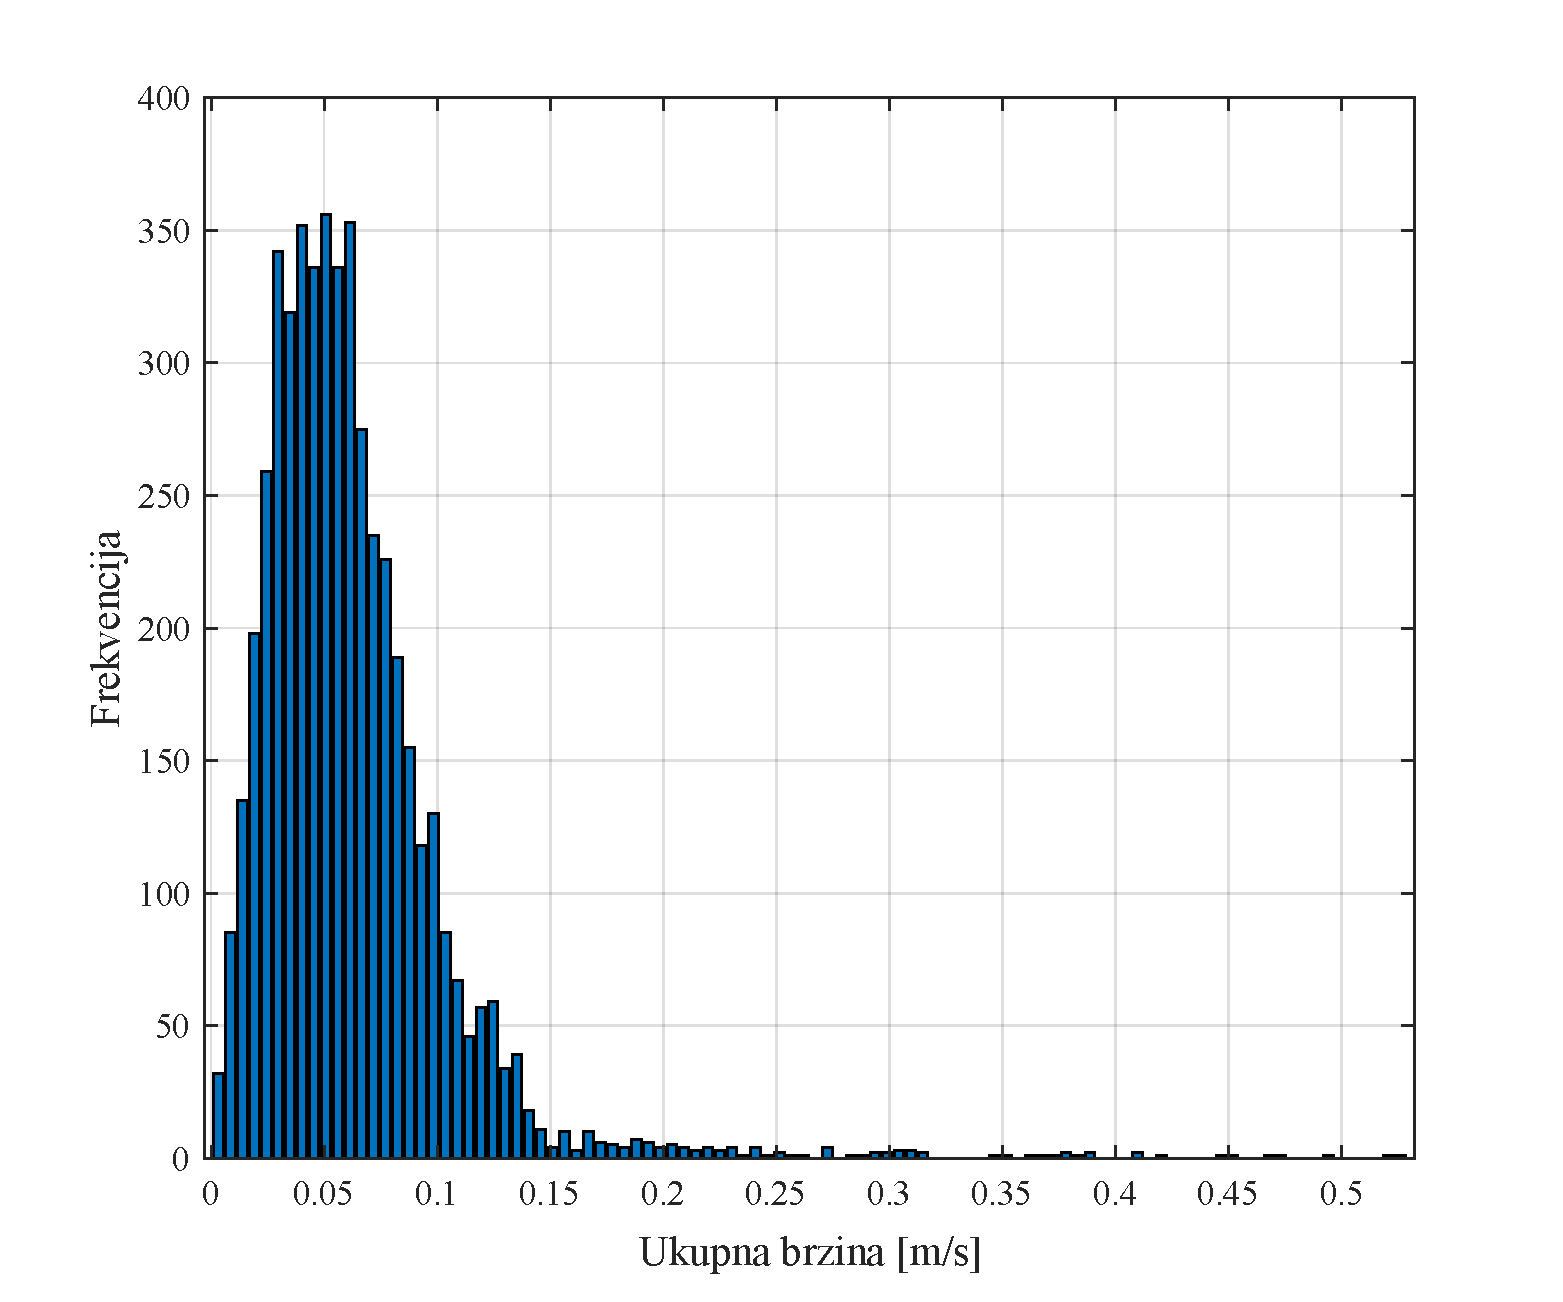
\includegraphics[width=10cm]{./7_LowCostPIV/slika7_11.pdf} 
	\caption{Dobiveni rezultati - Histogram svih ukupnih brzina strujanja u promatranoj domeni}
	\label{sl:7.11}
\end{figure}
